\documentclass{article}

% Page layout
\usepackage{geometry}
\geometry{
	a4paper,
}

% Fonts
\usepackage{fontspec}
\defaultfontfeatures{Mapping=tex-text,Scale=MatchLowercase}
\setmainfont{Linux Libertine O}

% Language
\usepackage{polyglossia}
\setdefaultlanguage{english}

% Graphics
\usepackage{graphicx}
\graphicspath{{./images/}}
\usepackage{dirtree}

% Links
\usepackage{url,hyperref}

% Headers and footers
\usepackage{fancyhdr}
\pagestyle{fancy}
\fancyhf{}
\lhead{
\includegraphics[scale=0.4]{inp-enseeiht}}
\rhead{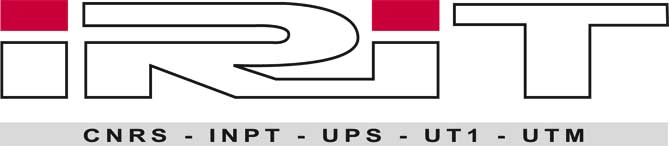
\includegraphics[scale=0.2]{irit}}
\lfoot{Install guide}
\rfoot{\bfseries \thepage}

% Code
\usepackage{verbatim}

\begin{document}

\sloppy

\vfill

\begin{center}
	{\Large Three-dimensional modelling and printing project}\\
	\bigskip
	{\Huge Install guide}\\
	\bigskip
	{\Large from January 23 to March 16, 2012}
\end{center}

\bigskip
\bigskip

\begin{center}
\large{
\textit{Vincent \textsc{Duvert} \\
Antoine \textsc{Lubineau} \\
Caroline \textsc{Naud} \\
James \textsc{Packer} \\
Florian \textsc{Ribon}} \\
\bigskip
INP-ENSEEIHT/IMA 
}
\end{center}

\vfill

\begin{figure}[!h]
\begin{center}
	
\includegraphics[scale=0.4]{inp-enseeiht}
\end{center}
\end{figure}

\bigskip

\begin{center}
http://www.enseeiht.fr/fr/index.html \\
2 Rue Charles Camichel \\
31 071 TOULOUSE
\end{center}

\vfill

\begin{figure}[!h]
\begin{center}
	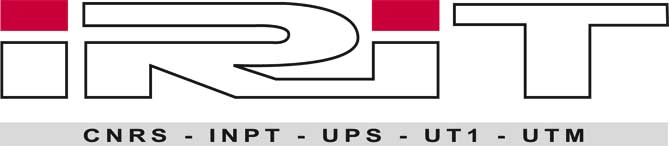
\includegraphics[scale=0.4]{irit}
\end{center}
\end{figure}

\begin{center}
http://www.irit.fr\\
Université Paul Sabatier \\
118 Route de Narbonne \\
F-31062 TOULOUSE CEDEX 9
\end{center}

\thispagestyle{empty}

\newpage

\tableofcontents

\newpage

\section{Global architecture of the application}

Here are (in orange) the different software and material you will have to get installed in order to use the complete application. The firmware is integrated in the printer and has not been modified in any way so you won't have to deal with it.

\begin{figure}[!h]
\begin{center}
	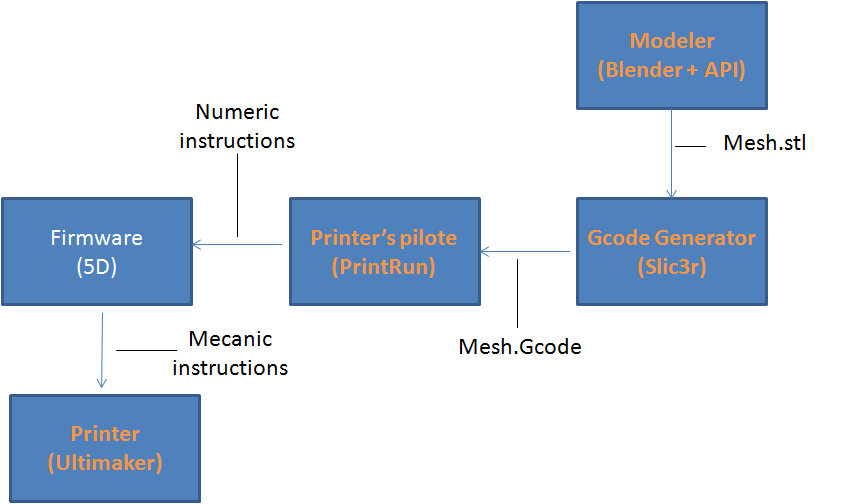
\includegraphics[scale=0.4]{ARD1}
\end{center}
\end{figure}

\newpage

\section{Installing Blender}

	\paragraph{Description} Blender is a free, open-source and multi-platform 3D modelling software.

	\paragraph{Homepage} \url{http://www.blender.org/}

	\paragraph{Recommended version} \textbf{2.50 and older} because we use the Python 3 API, but scripts were only tested from versions 2.58 to 2.62 (latest available). From version 2.63, Blender will include BMesh, a complete rewrite of some parts of the modelling engine; the main change will be the support of n-sided polygons (instead of triangles and quads currently). This might break some of our functions, as the API will also change. Progress on integration of BMesh can be seen here: \url{https://bmeshblender.wordpress.com/}.

	\paragraph{Windows} Download the latest version on \url{http://www.blender.org/download/get-blender/}.

	\paragraph{Linux} Providing your distribution has a recent version of Blender, you should use your package manager. Else, you can download the 32~bits or 64~bits on \url{http://www.blender.org/download/get-blender/}.

	\paragraph{MaxOS X} Go to \url{http://www.blender.org/download/get-blender/}. % TODO

\newpage

\section{Installing Slic3r}

	\paragraph{Description} Slic3r reads 3D models from STL files, and produces instructions for the printer as G-code (and M-code).

	\paragraph{Homepage} \url{http://slic3r.org/}

	\paragraph{Recommended version} \textbf{0.7.0 and older}, as it provides cooling support, better mesh slicing, binary compatibility with Ubuntu 11.10, etc.

	\paragraph{Windows} Go to \url{http://dl.slic3r.org/win/} and download \texttt{slic3r-mswin-x86-0-7-0.zip}. Extract the file, and you can launch \texttt{slic3r.exe} from the \texttt{Slic3r} folder.

	\paragraph{Linux} Go to \url{http://dl.slic3r.org/linux/} and download \texttt{slic3r-linux-x86-0-7-0.tar.gz}. To launch Slic3r:
		\begin{verbatim}
tar xz slic3r-linux-x86-0-7-0.tar.gz
cd Slic3r/bin
./slic3r
		\end{verbatim}

	\paragraph{MaxOS X} Go to \url{http://dl.slic3r.org/mac/} and download \texttt{slic3r-osx-uni-0-7-0.dmg}. % TODO

	\paragraph{Alternatives} Skeinforge is also one the most popular slicing software. It has many more options than Slic3r, and is divided in modules. In some cases, the code makes less visible wires outside the objects. Yet it is more difficult to configure (many settings are not obvious), and it is quite slow (it relies on Psyco, a Python accelerator which is not more actively supported). It is available on \url{http://fabmetheus.crsndoo.com/}.

\newpage

\section{Installing Blender plugin for printing and mesh preprocessing}

	\paragraph{Description} You should have an archive of those scripts.

	\paragraph{Windows} % TODO

	\paragraph{Linux} In \texttt{\~ {}/.blender/\emph{<version>}} (where \texttt{\emph{<version>}} is the Blender version you are using, such as \texttt{2.62}), put the \texttt{scripts} folder. Then copy \texttt{startup.blend} in a \texttt{config} directory (it may or may not exist). You should have the following directory structure:\\

\dirtree{%
 .1 .blender.
 .2 <version>.
.3 config.
.4 startup.blend.
.3 scripts.
.4 modules.
.5 \_\_init\_\_.py.
.5 holes.py.
.5 manifold.py.
.5 planar\_faces.py.
.5 volume.py.
.4 run\_tests.sh.
.4 startup.
.5 printing\_preprocessing.py.
.4 tests.
.5 \_\_init\_\_.py.
.5 all.py.
.5 test\_manifold.py.
.5 test\_planar\_faces.py.
.5 utils.py.
}

	\paragraph{MacOS X} % TODO

	Once everything is installed, every time you start Blender, you should have a customized interface, with a new panel in the object editor, “Mesh verification”.

\newpage

\section{Installing Printrun}

	\paragraph{Description} Printrun is an interface for uploading G-code to the printer, and for manual piloting. One can also visualize the G-code in realtime while the object is printed.

	\paragraph{Home page} \url{https://github.com/kliment/Printrun}

	\paragraph{Installation} Instructions are available on \url{https://github.com/kliment/Printrun}.

	\paragraph{Alternatives} ReplicatorG is also very used with 3D printers; it is available on \url{http://replicat.org/}.

\end{document}
